\documentclass[10pt,mathserif]{beamer}
\usepackage{graphicx,amsmath,amssymb,tikz,psfrag}
\usepackage{hyperref}
%\usepackage{graphicx,psfrag}

\input defs.tex
\input slide_format.tex

%% begin presentation

\title{\large \bfseries Discovering signals in fMRI data; 
a Bayesian nonparametric approach }

\author{Ahmed Bou-Rabee, Wanrong Zhu, Zheng Xu, Mo Zhou\\[3ex]
Stats 308\\
University of Chicago}

\date{\today}

\begin{document}

\frame{
\thispagestyle{empty}
\titlepage
}

\begin{frame} {What is fMRI data?}
\BIT
\item  
\item 
\EIT
\end{frame}

\begin{frame} {What's our method}
\BIT
\item  
\item 
\EIT
\end{frame}

\begin{frame} {Details of method}
\BIT
\item  introduce the talk 
\item 
\EIT
\end{frame}

\begin{frame} {Performance on toy data}
\BIT
\item  introduce the talk 
\item 
\EIT
\end{frame}

\begin{frame} {Performance on real fMRI data}
\BIT
\item  introduce the talk 
\item 
\EIT
\end{frame}



\begin{frame}{comparison to p-filter}
\begin{center}
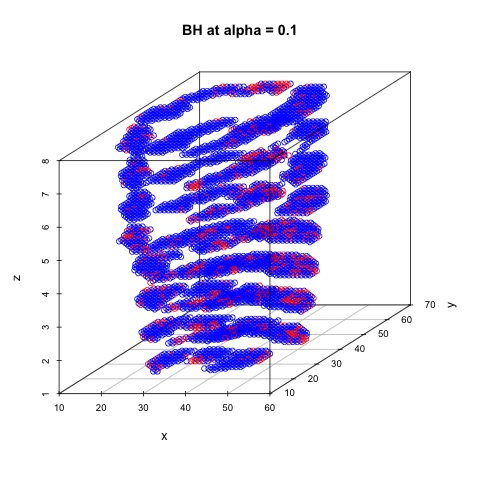
\includegraphics[height=0.35\textheight]{../BH_predictions.jpg} \\ 
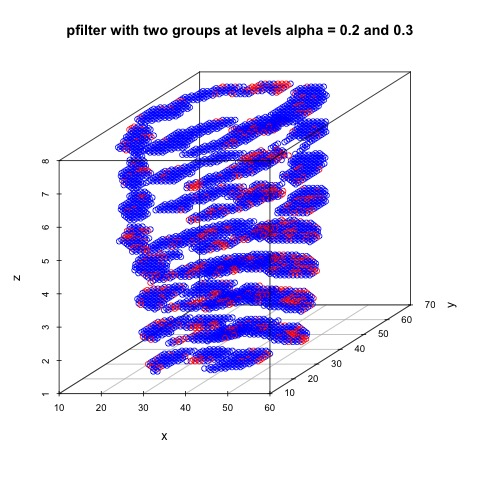
\includegraphics[height=0.35\textheight]{../pfilter_predictions.jpg} \\ 
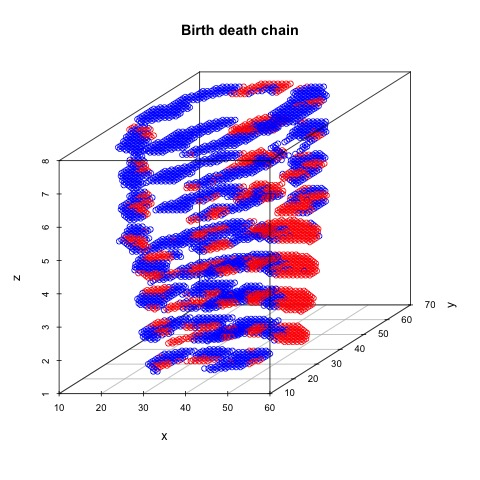
\includegraphics[height=0.35\textheight]{../BDC_predictions.jpg} \\ 
\end{center}
\end{frame}

\end{document}
